% =============================================================================
% COLING 2027 submission — ACL two-column, 8-page long paper, anonymized.
%
% Repositioning: "LLM agent memory rollback security" -> "trustworthy inference
% over natural-language agent memory": the story is now about natural-language
% memory, retrieval, answer recovery (generation/QA), and cross-lingual recall.
% Security/threat-model language is weakened in favor of memory robustness.
%
% Build notes:
%  * Requires acl.sty (ACL/COLING style file) and acl_natbib.bst. Download from
%    https://acl-org.github.io/ACLPUB/ (style files). The preamble below follows
%    the standard ACL template (\documentclass[11pt]{article} + \usepackage{acl}).
%  * ANONYMOUS: no \author block, no acknowledgments, no self-citations.
%    Uncomment \aclfinalcopy and add \author{...} only for the camera-ready.
%  * Figures referenced below are in C:/Users/acer/agent-sec-graph/figures/ as
%    .svg/.png; convert the SVGs to PDF/PNG before the camera-ready build.
% =============================================================================

\documentclass[11pt]{article}

% --- ACL style -----------------------------------------------------------------
\usepackage{acl}            % ACL/COLING two-column style (download acl.sty)
% \aclfinalcopy             % uncomment ONLY for camera-ready (adds running header)

% --- Fonts / encoding ----------------------------------------------------------
\usepackage[T1]{fontenc}
\usepackage[utf8]{inputenc}
\usepackage{times}
\usepackage{latexsym}
\usepackage{microtype}
\usepackage{inconsolata}

% --- Math / tables / figures ---------------------------------------------------
\usepackage{amsmath,amssymb,amsthm}
\usepackage{booktabs}
\usepackage{graphicx}

% --- Citations -----------------------------------------------------------------
% NOTE: acl.sty already issues \RequirePackage{natbib} and
% \bibliographystyle{acl_natbib}; declaring the style again here would duplicate the
% \bibstyle line in the .aux and make BibTeX fail with "another \bibstyle command".
\usepackage{natbib}

% --- Theorem-like environments -------------------------------------------------
\newtheorem{theorem}{Theorem}
\newtheorem{lemma}{Lemma}
\newtheorem{proposition}{Proposition}
\newtheorem{definition}{Definition}
\theoremstyle{remark}
\newtheorem{remark}{Remark}

% --- Macros --------------------------------------------------------------------
\newcommand{\ours}{\textsc{ProvRepair}}
\newcommand{\anchor}{provenance-only baseline}
\newcommand{\sbed}{\textsc{SB-ED}}
\newcommand{\dlbp}{\textsc{DL-BP}}
\newcommand{\csr}{\textsc{CS-R}}

\title{Faithful Answers from Incomplete Memory:\\ Provably Complete Recovery of Natural-Language Agent Memory}

% ====== ANONYMIZED: no authors, no institutions, no acknowledgments =============
% \author{Anonymized submission}

\begin{document}

\maketitle

\begin{abstract}
Language agents write natural-language notes, persist them across sessions, and later
retrieve them to answer questions. When a note goes stale, contradicts a newer value, or
is written under the influence of unreliable content, the retrieved memory silently steers
downstream generation---and the corruption survives, because the agent records its own
causal history only partially. We show that faithful answer recovery is an
\emph{inverse-reconstruction} problem: the recorded provenance graph is a lossy,
corruptible encoding of the true history, so recovery is complete exactly when provenance
is complete. This completeness fails in four orthogonal, exhaustive ways---a missing
derivation edge, a missing root, poisoned content, and a spurious edge---one of which (the
out-of-trace root) is provably uncloseable from the trace alone. We present \ours, which
closes all four with three operators: budgeted semantic edge inference, a dual-layer
consistency fixed point, and version-history value restoration. On 1{,}264 synthetic cases
and 451 real LongMemEval-V2 trajectories, \ours\ closes all four gaps (451/451 vs.\ 0/451
for a \anchor) and lifts answer recovery from 4--24\% to 76--92\% across three models; a
multilingual retriever (\textsc{bge-m3}) closes the cross-lingual blind spot, raising
derivation recall from 0/15 to 15/15.
\end{abstract}

\section{Introduction}

Memory-augmented language agents \citep{park2023generative,packer2023memgpt,zhong2024memorybank}
reason over \emph{natural-language memory}: across
turns they read notes, act, and write new notes that persist to later sessions. The
memory store is not a passive log but a retrieval index
\citep{lewis2020rag,karpukhin2020dpr}---a later answer is generated
from whatever the store returns---so the trustworthiness of an agent's reasoning
reduces to the trustworthiness of its retrieved memory. Memory is therefore a
first-class object of study for NLP: it is generated, retrieved, and paraphrased, and
its failures are linguistic---a note that omits its source, a merge whose summary
drifts, a fact value rewritten in a single letter.

But natural-language memory is fragile. A note may be \emph{stale}, may contradict a
newer value, or may be written under the implicit influence of unreliable content read
in an earlier session. Because the agent records its own history imperfectly, such a
note is retrieved later and silently steers generation; the corruption is not
transient but \emph{sedimented} into the store, and it keeps acting long after the
triggering content is gone. Recovering the faithful answer therefore requires more
than deleting the offending note: every derived note that inherited the corruption
must be found and repaired, and the correct value restored. This is the problem we
study.

\begin{figure}[t]
\centering
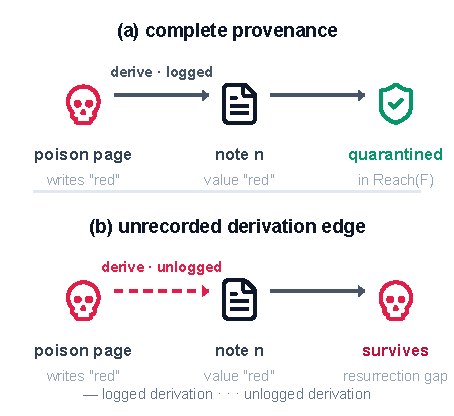
\includegraphics[width=\columnwidth]{figure1_teaser_tight}
\caption{The residual-contamination gap: a note derived from a poisoned page is
quarantined when its derivation edge is logged (a), but survives rollback when the edge
is unlogged (b).}
\label{fig:teaser}
\end{figure}

We approach it through a single principle. \textbf{Memory recovery is the
reconstruction of a lossy encoding.} The provenance graph an agent's runtime records
---who wrote which note, and which note was derived from which---is a lossy,
corruptible encoding of the true causal history. Recovery is therefore not a deletion
that removes a fault's reachable set, but an \emph{inverse reconstruction} that
recovers the true contamination closure from this encoding; and any inverse
reconstruction is bounded by the information the encoding retains. Hence \emph{recovery completeness
equals provenance completeness} (Lemma~\ref{lem:complete}): when a derivation edge goes
unrecorded---the agent wrote a note under implicit influence without citing its
source---the derived note becomes invisible to graph reachability and survives the
recovery. We call this the \emph{residual-contamination gap}.

We prove that this incompleteness takes exactly four orthogonal, exhaustive forms: a
\emph{missing derivation edge}, a \emph{missing root}, \emph{poisoned content}, and a
\emph{spurious edge} (Theorem~\ref{thm:four}). One of them, the out-of-trace root, is
the unique dimension no in-trace operator can close (Theorem~\ref{thm:impossibility}):
its correct value was produced in an earlier session absent from the trace, and no
graph completion reconstructs it. This classification turns the question ``can memory
recovery be complete?'' into a provable question about whether four encoding losses
can be eliminated, each requiring a \emph{different} repair.

We present \ours, which closes the four dimensions with three operators.
\emph{Budgeted semantic edge inference} (\sbed) recovers missing derivation edges
under a verification budget with a provable $(1{-}1/e)\cdot\alpha$ bound; a
\emph{dual-layer belief-propagation fixed point} (\dlbp) corrects poisoned content and
revokes spurious edges; and \emph{version-history value restoration} (\csr) restores
out-of-trace roots. Together they are complete up to a single measurable knob---the
inference recall (Theorem~\ref{thm:recall})---rather than an uncontrolled structural
gap.

Across 1{,}264 synthetic cases and 451 real LongMemEval-V2 trajectories, \ours\ closes
all four gaps (451/451 vs.\ 0/451 for a \anchor) and lifts answer recovery from
4--24\% to 76--92\% across three models (\texttt{deepseek-v4-pro},
\texttt{qwen3.7-plus}, \texttt{claude-sonnet-5}). A multilingual retriever
(\textsc{bge-m3}) closes the cross-lingual blind spot, raising derivation recall from
0/15 to 15/15. Our contributions are:

\begin{itemize}
\itemsep0pt
\item \textbf{A completeness law and its exhaustive decomposition.} We formalize
memory recovery as the reconstruction of a lossy encoding, prove recovery
completeness equals provenance completeness, and decompose its failure into four
orthogonal, exhaustive dimensions (Theorem~\ref{thm:four}), each needing a distinct
repair.
\item \textbf{An impossibility boundary.} We prove the out-of-trace root is the unique
dimension no in-trace operator can close (Theorem~\ref{thm:impossibility}), which
mechanistically explains why \emph{stale} records recur far more often than
\emph{injected} ones in prior rollback work.
\item \textbf{A complete three-operator recovery.} \ours\ closes all four dimensions
with three operators (\sbed, \dlbp, \csr), relegating probabilistic judgment to a
bounded fallback and achieving completeness up to a single measurable recall knob
(Theorem~\ref{thm:recall}).
\item \textbf{Empirical closure.} On 1{,}264 synthetic cases and 451 real trajectories,
\ours\ closes all four gaps and lifts answer recovery from 4--24\% to 76--92\%.
\end{itemize}

\section{Related Work}
\label{sec:related}

\paragraph{Language agents and memory.} Tool-using and reasoning agents
\citep{schick2023toolformer,yao2022react} ground their behavior in an
external memory of natural-language notes, spanning generative simulators
\citep{park2023generative}, OS-style memory hierarchies \citep{packer2023memgpt}, and
structured long-term stores \citep{zhong2024memorybank,modarressi2024memoryllm}. The store is
a retrieval index in the lineage of retrieval-augmented generation
\citep{lewis2020rag,karpukhin2020dpr,izacard2021fid,guu2020realm,borgeaud2022retro}, so its
failures---stale notes, drifting merges, paraphrased sources---are retrieval-faithfulness
failures of the kind studied in RAG evaluation \citep{gao2023ragsurvey,chen2023rgb,es2023ragas}.
We study the recovery side: given a faulty store, repair every derived record that inherited
the corruption.

\paragraph{Poisoning, injection, and defense.} Poisoning work plants corrupted knowledge or
memories \citep{chen2024agentpoison,zou2025poisonedrag,dong2025minja,huang2024memorysandbox,graftgraph2026};
prompt-injection work studies how untrusted content steers a model at the interface
\citep{greshake2023not,perez2022ignore,liu2023promptinjection}, and agent-security benchmarks
formalize the threat \citep{zhang2024asb,debenedetti2024agentdojo,toyer2024tensortrust}.
Detection and prevention filter or structure inputs before they act
\citep{liu2025datasentinel,chen2025struq}, and persistent-control work shows a single injection
can be sedimented into durable control \citep{yang2026zombie}. The long-term-memory survey
\citep{lin2026survey} names ``residual derivatives after deletion'' as an open gap.

\paragraph{Recovery and repair.} Version rollback \citep{su2026chronomem,zheng2026acrfence},
cascade invalidation
\citep{zhao2026memorepair}, and dependency-guided rollback \citep{yu2026dependency} trace
contamination over a provenance graph and deactivate its reachable set; Yu et al.\ report a
recurrence anomaly---\emph{injected} records recur at $0.000$ while \emph{stale} records recur
at $0.781$---which \S\ref{sec:four} mechanistically explains. All of these assume the provenance
graph they roll back over is \emph{complete}; we show that assumption fails in exactly four
orthogonal ways and repair each. Model-editing work \citep{meng2022rome,mitchell2022mend}
edits a single model's parameters in place; we instead restore the correct \emph{value} over a
provenance graph. Closest in spirit are benchmarks
\citep{memsecbench2026,purgebench2026,wu2024longmemeval} that identify provenance as the
decisive lever against re-emergence, and the Assured-Intelligence architecture
\citep{assuredintelligence2026}, which states completeness as a single precondition; we
decompose it exhaustively and prove one dimension is uncloseable in-trace.

\section{Threat Model}
\label{sec:threat}

We state the threat model precisely: what memory is, how it is recorded, and the four
exhaustive ways in which that recording can fail.

\subsection{Memory as a Lossy Encoding}
\label{sec:formulation}

\begin{definition}[Provenance graph]
An agent's trace induces a typed graph $G=(V,E)$ over memory records, execution
steps, and user inputs, with edges such as \texttt{cite}, \texttt{produce},
\texttt{derive}, \texttt{update}, and \texttt{supersede}. The true causal graph is
$G^{*}=(V^{*},E^{*})$; the runtime records only a subset of nodes and edges, $V\subseteq V^{*}$ and $E\subseteq E^{*}$.
Derivation edges under implicit influence, prior-session producing edges, and the
content--provenance alignment of a merge may each go unrecorded. For a set $F$ of
diagnosed faulty records, the true contamination closure is $\mathcal{H}^{*} =
\mathrm{Reach}_{G^{*}}(F)$ and the recorded one is $\mathcal{H} =
\mathrm{Reach}_{G}(F)$, where reachability follows propagation edges.
\end{definition}

Recovery is \emph{distortion-free} iff it removes exactly the true closure and
preserves correct content: $\mathcal{H}=\mathcal{H}^{*}$ and every shared record
carries its true value.

\begin{lemma}[Recovery completeness = provenance completeness]
\label{lem:complete}
A recovery over the recorded graph is complete---it removes every truly contaminated
record---if and only if every contamination edge is recorded, i.e.\
$E^{*}_{\mathrm{prop}}\subseteq E_{\mathrm{prop}}$.
\end{lemma}

\begin{proof}[Proof sketch]
Reachability is monotone in the edge set, so recording all edges implies the closure
is complete; conversely, a single unrecorded edge on a contamination path hides the
record behind it from reachability.
\end{proof}

Lemma~\ref{lem:complete} is an information-theoretic law specialized to provenance:
the completeness of any inverse reconstruction is bounded by what the encoding
retains.

\subsection{Four Orthogonal Failure Modes}
\label{sec:four}

The distortion $\Delta = (\mathcal{H}^{*}\setminus\mathcal{H}) \cup
(\mathcal{H}\setminus\mathcal{H}^{*}) \cup \{v\in\mathcal{H}^{*}\cap\mathcal{H}:
\hat\lambda(v)\ne\lambda(v)\}$ admits an exhaustive decomposition.

\begin{theorem}[Exhaustive classification]
\label{thm:four}
Every non-empty distortion is caused by one of four orthogonal deviations of $G$ from
$G^{*}$: (1)~\emph{missing edge}---a true derivation edge unlogged; (2)~\emph{missing
root}---a true ancestor absent from the trace; (3)~\emph{content error}---a shared
record whose label is corrupted; (4)~\emph{spurious edge}---an observed edge absent
from the truth. A ``phantom node'' reduces to a spurious edge, so no fifth dimension
exists.
\end{theorem}

\begin{proof}[Proof sketch]
$\Delta$ is a disjoint union of three sets: a true ancestor missing from the observed
closure is either absent from $V$ (dimension~2) or has a true edge missing on its
path (dimension~1); an observed ancestor absent from the true closure has a spurious
edge on its path (dimension~4); the content term is dimension~3. Each set is non-empty
iff its dimension is violated, so the four dimensions form a disjoint, exhaustive
basis. A mechanical enumerator over all single-point graph edits confirms each edit
lands in exactly one dimension.
\end{proof}

\begin{figure}[t]
\centering
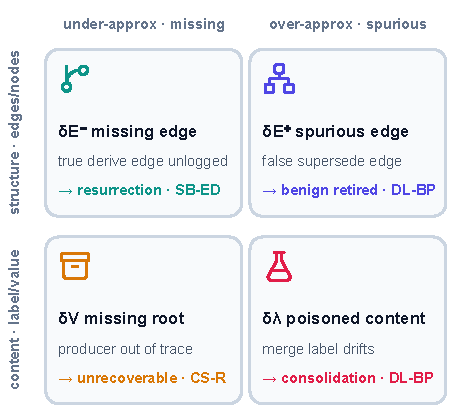
\includegraphics[width=\columnwidth]{figure2_4dim_coordinate_tight}
\caption{The four orthogonal failure modes of Theorem~\ref{thm:four} in coordinate form,
arranged by structure vs.\ content and under- vs.\ over-approximation.}
\label{fig:fourdim}
\end{figure}

Table~\ref{tab:fourdims} maps each dimension to the linguistic phenomenon that causes
it and to the repair that closes it.

\begin{table*}[t]
\centering
\small
\begin{tabular}{llll}
\toprule
\textbf{Dimension} & \textbf{Linguistic source} & \textbf{Gap} & \textbf{Repair} \\
\midrule
Missing edge & implicit influence, source uncited & residual contamination & \sbed\ (edge inference) \\
Missing root & stale value produced in a prior session & unrecoverable value & \csr\ (version history) \\
Content error & merge summary drifts from its clean source & poisoned summary & \dlbp\ semantic pass \\
Spurious edge & unreliable supersession retires a trusted note & silent value loss & \dlbp\ topological pass \\
\bottomrule
\end{tabular}
\caption{The four orthogonal failure modes of Theorem~\ref{thm:four}, the natural-language
phenomenon that causes each, and the operator that closes it.}
\label{tab:fourdims}
\end{table*}

\begin{theorem}[Impossibility of in-trace root recovery]
\label{thm:impossibility}
The missing root is the unique dimension no in-trace operator can close: if a faulty
record has no producing step in $V$, its correct value was produced in a prior session
absent from $G$, and no graph completion over $G$ alone reconstructs it.
\end{theorem}

\begin{proof}[Proof sketch]
Two ground truths that differ only in the absent value induce the same observed graph,
so any algorithm that sees only $G$ must output the same value on both and errs on one.
\end{proof}

Theorem~\ref{thm:impossibility} mechanistically explains why \emph{stale} records recur
far more often than \emph{injected} ones in prior rollback work (the recurrence contrast
is quantified in \S\ref{sec:related}): injected records have an in-trace producer that
can be replayed, whereas a stale record's correct value is produced out of trace and
cannot be.

\section{Approach}
\label{sec:approach}

\begin{figure*}[t]
\centering
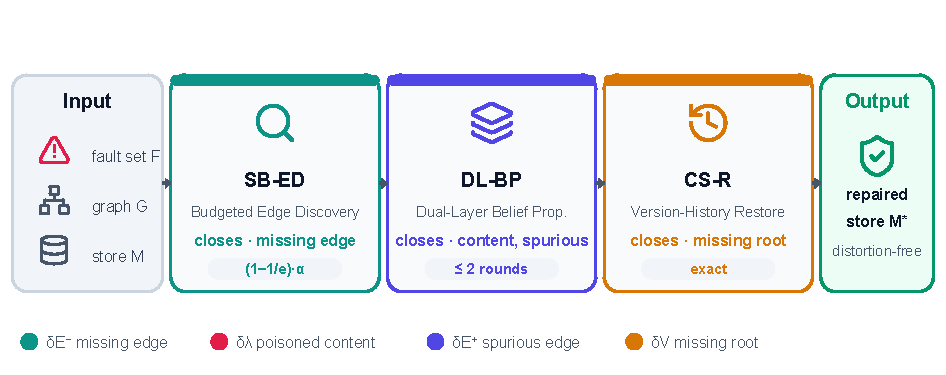
\includegraphics[width=\textwidth]{figure3_framework_tight}
\caption{The \ours\ framework: three operators (\sbed, \dlbp, \csr) close the four
failure dimensions between diagnosed faults and a restored clean store.}
\label{fig:framework}
\end{figure*}

\subsection{Three Operators}
\label{sec:operators}

\paragraph{\sbed\ (missing edge).} Candidate derivation edges are filtered by temporal
monotonicity and a semantic prior
$\mathcal{C}=\{(u,v): \mathrm{Session}(v)\ge\mathrm{Session}(u) \wedge
\cos(\mathbf{x}_u,\mathbf{x}_v)\ge\theta_{\mathrm{sim}} \wedge (u,v)\notin E\}$. Under
a verification budget $B$, a greedy pass adds the edge of maximum marginal coverage of
the contamination closure; a verifier confirms each candidate. The coverage objective
is monotone submodular, so the greedy attains $(1{-}1/e)$ under a perfect oracle and
$(1{-}1/e)\cdot\alpha$ under an imperfect two-stage oracle with effective recall
$\alpha$ (Nemhauser--Wolsey--Fisher; \citep{nemhauser1978submodular,krause2014submodular}).

\paragraph{\dlbp\ (content error, spurious edge).} A justified-belief truth-maintenance
system \citep{doyle1979tms,dekleer1986atms} runs a dual-layer fixed point over the memory-state lattice
$\{\textsc{Active},\textsc{Superseded},\textsc{Quarantined}\}$ with a suspicion score
$\tau_v$. The \emph{semantic pass} quarantines a merged record whose content diverges
from every clean parent (closing content error); the \emph{topological pass} revokes a
supersession authored by an unreliable source (closing the spurious edge); a third step
unwinds premature evictions when a quarantined record's clean support is re-established.
The iteration stabilizes in at most two rounds on every trace.

\paragraph{\csr\ (missing root).} For a root fault the correct value is out of trace, so
\csr\ substitutes the latest clean snapshot from version history \emph{in place},
inheriting the fault's causal identity so no downstream derivation edge is severed.

\begin{theorem}[Completeness up to the recall knob]
\label{thm:recall}
\dlbp\ and \csr\ close their dimensions exactly; \sbed\ is the only approximate closure,
recovering each missing edge with recall $\rho_e$. The only residual contamination is
that reachable solely through a derivation edge \sbed\ missed, bounded by
$\Pr[\text{survive}]\le 1-\min_{p\in\mathrm{Paths}_{G^{*}}(F,v)}\prod_{e\in p}c_e$,
where $c_e{=}1$ for a recorded edge and $c_e{=}\rho_e$ for a missing edge recovered with recall $\rho_e$. When $\rho_e{=}1$ on every contamination path the bound vanishes;
otherwise completeness degrades by exactly the measurable recall $\rho_e$.
\end{theorem}

\section{Experimental Setup}
\label{sec:setup}

\textbf{Datasets.} 1{,}264 synthetic cases (5 domains $\times$ 4 fault types:
injected, stale, misattributed, summary-drift), programmatically generated and seeded;
451 real LongMemEval-V2 trajectories \citep{wu2024longmemeval,wu2026longmemeval}, each anchored to a real
trace and injecting one of the four gaps over the question's ground-truth answer; and
two production memory engines (Mem0, Graphiti) for deployment checks.

\textbf{Models.} \texttt{deepseek-v4-pro}, \texttt{qwen3.7-plus},
\texttt{claude-sonnet-5} for end-to-end answer recovery; local open-source models
(\texttt{qwen3:8b}, \texttt{qwen2.5:7b}) for derivation-gap measurement.

\textbf{Metrics.} Following prior rollback work \citep{yu2026dependency}, we report
residual contamination (re-emergence), value restoration, contamination leak,
benign loss, and replay ratio (the re-generation cost), plus Wilson 95\% intervals.
We separate deterministic memory-set metrics (which isolate correctness from model
stochasticity) from end-to-end answer recovery via live replay.

\textbf{Baselines.} Naive Deletion, Checkpoint Restore (\citet{su2026chronomem}),
Cascade Invalidation (\citet{zhao2026memorepair}), Dependency-Guided Rollback
(\citet{yu2026dependency}, the \anchor), Global Re-execution (oracle), a content-only
LLM judge, and four adapted write-stage/information-flow defenses, including stale-memory
revocation (TEPA, \citet{tepa2026}) and recoverable information-flow control (APPA,
\citet{kravchenko2026appa}).

\section{Results}
\label{sec:results}

\subsection{Four-Dimension Closure}
\label{sec:closure}

Table~\ref{tab:closure} reports closure on the synthetic pool and the real
trajectories. The \anchor\ closes none of the four gaps; \ours\ closes all four on
both settings.

\begin{table}[t]
\centering
\small
\begin{tabular}{lc}
\toprule
\textbf{Gap} & \textbf{Synthetic closure} \\
\midrule
Missing edge & 1264/1264 $\to$ \textbf{0} \\
Missing root & 0/632 $\to$ \textbf{632/632} \\
Poisoned content & 316/316 $\to$ \textbf{0} \\
Spurious edge & 316/316 $\to$ \textbf{0} \\
\bottomrule
\end{tabular}
\caption{Four-dimension closure on the 1{,}264-case synthetic pool (\anchor\ $\to$ \ours);
rows report resurrection, root restoration, content leak, and benign loss, respectively.
On 451 real LongMemEval-V2 trajectories, \ours\ closes all four gaps (451/451 vs.\ 0/451
for the \anchor).}
\label{tab:closure}
\end{table}

\subsection{Answer Recovery}
\label{sec:answer}

The headline result is end-to-end \emph{answer recovery}: after a faulty memory is
repaired, does the agent generate the correct answer? On 51 value-fault trajectories
(a deleted root value and a poisoned summary), the \anchor\ recovers the answer in
4--24\% of cases---model-dependent guessing from an empty or poisoned store---while
\ours\ restores the correct value and lifts every model to 76--92\%
(Table~\ref{tab:answer}). A McNemar paired test gives $\chi^2=34$--$43$ ($p<0.001$).

\begin{figure}[t]
\centering
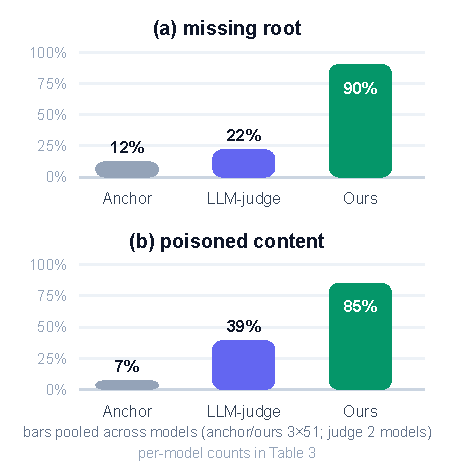
\includegraphics[width=\columnwidth]{figure4_answer_recovery_tight}
\caption{Answer recovery on 51 value-fault trajectories, comparing the \anchor, a
content-only LLM judge, and \ours across two fault types (missing root and poisoned
content).}
\label{fig:answer}
\end{figure}

\begin{table}[t]
\centering
\footnotesize
\begin{tabular}{lcc}
\toprule
\textbf{Model} & \textbf{Missing root} & \textbf{Poisoned content} \\
\midrule
\texttt{deepseek-v4-pro} & 5/51 $\to$ \textbf{47/51} & 4/51 $\to$ \textbf{47/51} \\
\texttt{qwen3.7-plus} & 12/51 $\to$ \textbf{47/51} & 2/51 $\to$ \textbf{44/51} \\
\texttt{claude-sonnet-5} & 2/51 $\to$ \textbf{44/51} & 5/51 $\to$ \textbf{39/51} \\
\midrule
Aggregate & \multicolumn{2}{c}{4--24\% $\to$ \textbf{76--92\%}} \\
\bottomrule
\end{tabular}
\caption{Answer recovery on 51 value-fault trajectories (each cell reports \anchor\ $\to$ \ours, correct-answer fraction). \ours\ restores the value and lifts every model to 76--92\%.}
\label{tab:answer}
\end{table}

\subsection{Baseline Comparison}
\label{sec:baseline}

Table~\ref{tab:baseline} scores 11 methods on five dimensions over
weakness-targeting scenarios. No two rows are identical; the content-only LLM judge
(a real DeepSeek run) is far stronger than a lexical proxy but still resurrects 2.3\%
of cases exactly where provenance is the only signal. Global Re-execution and \ours\
share the four correctness dimensions but split on replay ratio (1.00 vs.\ 0.90):
\ours\ reaches oracle-tier closure at \anchor-tier cost.

\begin{table*}[t]
\centering
\small
\begin{tabular}{lccccc}
\toprule
\textbf{Method} & \textbf{Resurr.} $\downarrow$ & \textbf{Root rec.} $\uparrow$ & \textbf{Poison leak} $\downarrow$ & \textbf{Over-del.} $\downarrow$ & \textbf{Replay} $\downarrow$ \\
\midrule
Naive Deletion & 100\% & 0\% & 20\% & 0\% & 0.00 \\
Checkpoint Restore (ChronoMem) & 0\% & 0\% & 40\% & 33\% & 0.00 \\
Cascade Invalidation (MemoRepair) & 0\% & 0\% & 0\% & 33\% & 0.90 \\
Anchor (Yu 2026) & 0\% & 0\% & 20\% & 0\% & 0.90 \\
Global Re-exec (oracle) & 0\% & 100\% & 0\% & 0\% & 1.00 \\
LLM judge (DeepSeek, content-only) & 2.3\% & 0\% & 0.06\% & 0\% & 0.00 \\
MemLineage-adapt & 17\% & 0\% & 20\% & 33\% & 0.00 \\
MAP-Graph-adapt & 83\% & 0\% & 80\% & 0\% & 0.00 \\
TEPA-adapt & 83\% & 50\% & 80\% & 0\% & 0.90 \\
APPA-adapt & 0\% & 50\% & 20\% & 0\% & 0.90 \\
\ours\ (full) & \textbf{0\%} & \textbf{100\%} & \textbf{0\%} & \textbf{0\%} & \textbf{0.90} \\
\bottomrule
\end{tabular}
\caption{Eleven methods on five dimensions over weakness-targeting scenarios.
Denominators: resurrection 1{,}896, root recovery 632, poison leak 1{,}580,
over-deletion 948. The LLM-judge row is a real DeepSeek run, not a lexical proxy.
\ours\ reaches oracle-tier closure at \anchor-tier replay cost (0.90 vs.\ 1.00).}
\label{tab:baseline}
\end{table*}

\subsection{Derivation-Inference Recall Ladder}
\label{sec:recall}

The completeness of \sbed\ is governed by the recall $\rho_e$ with which it recovers
paraphrased derivations---an NLP-sensitive quantity. Table~\ref{tab:ladder} shows the
recall ladder on 15 real derivations: lexical token overlap has zero recall (a real
agent \emph{rewrites} rather than copies); embedding cosine (nomic-embed-text) reaches
13/15; base64-decode normalization reaches 14/15; and the multilingual embedder
\textsc{bge-m3} \citep{chen2024bgem3} closes the cross-lingual blind spot (cross-lingual
cosine 0.45 $\to$
0.82), reaching 15/15. This is the measurable knob behind Theorem~\ref{thm:recall}.

\begin{table}[t]
\centering
\small
\begin{tabular}{lc}
\toprule
\textbf{Inference signal} & \textbf{Recall (15 derivations)} \\
\midrule
Lexical token overlap & 0/15 \\
Embedding cosine & 13/15 \\
$+$ base64 decode & 14/15 \\
Multilingual & \textbf{15/15} \\
\bottomrule
\end{tabular}
\caption{The derivation-inference recall ladder (embedders: nomic-embed-text for cosine, \textsc{bge-m3} for multilingual). Multilingual \textsc{bge-m3} closes the cross-lingual blind spot, reaching 15/15.}
\label{tab:ladder}
\end{table}

\subsection{Ablation and Diagnosis Robustness}
\label{sec:ablation}

\textbf{Ablation.} Removing \sbed\ reopens the missing-edge dimension (resurrection
returns to 1264/1264); removing the \dlbp\ fixed point reopens premature eviction
(over-deletion returns to 100/100); removing \csr\ drops root recovery to 0/632. Each
ablation reopens exactly its own dimension, so the three operators are minimal and
non-redundant.

\textbf{Imperfect diagnosis.} Injecting missed diagnosis (false negatives) drives
structural residual contamination linearly from 0\% to 50\%; false positives drive
benign loss from 0\% to 63\%. Neither amplifies, and the content dimension stays at
0\% under missed diagnosis because the content-consistency check is a provenance-free
full pass independent of the diagnosis seed.

\section{Conclusion}

Memory recovery is correct exactly when provenance is complete; that incompleteness has
exactly four orthogonal forms; and \ours\ closes all four with three operators,
compressing the residual distortion to a measurable recall bound. What prior work
reports as an unexplained recurrence anomaly becomes a property that is provable,
diagnosable, and repairable---so that a language agent's answer is faithful to the
history it actually lived, not merely to what its store happened to keep.

\section{Limitations}
\label{sec:limitations}

(1)~\textbf{Upper-bound synthetic cases.} The single-fault synthetic pool carries no
benign \emph{derived} memory to cascade away, so its 0\% benign loss is a construction
artifact; the real over-deletion difference appears only in the multi-fact setting and
the fixpoint ablation. (2)~\textbf{Model coverage.} \texttt{GPT-4o} and \texttt{Gemini}
were not run, and the reasoning model was too slow for the content-only judge baseline,
which uses two non-reasoning models. (3)~\textbf{Cross-session fidelity.} The
out-of-trace root is encoded via template injection rather than a full two-session
harness, though a cross-agent experiment partially covers this. (4)~\textbf{Content
granularity.} The content-consistency check uses exact fact-value matching because
embedding cosine cannot separate single-letter value differences---a mechanism choice,
not a defect. (5)~\textbf{Diagnosis oracle.} The faulty-record set is supplied by an
orthogonal detector; robustness to imperfect diagnosis is quantified in
\S\ref{sec:ablation} but end-to-end detection remains outside scope. (6)~\textbf{Scope
of cross-lingual result.} The \textsc{bge-m3} recall gain is demonstrated on 15
derivations; larger multilingual coverage remains for future work.

\section{Ethical Considerations}
\label{sec:ethics}

This work studies how to recover faithful answers from corrupted agent memory. It uses
only synthetic cases and the public \textsc{LongMemEval-V2} benchmark; no human subjects,
personal data, or user interactions are involved. The memory-poisoning techniques we
describe exist to characterize the failure modes of memory-augmented agents
\emph{defensively}: our goal is repair, not attack. We acknowledge a dual-use
consideration---the same provenance-recovery machinery could in principle be used to
target a store more precisely---but we regard faithful recovery as strictly beneficial,
since it makes a model's answer depend on the history it actually lived rather than on
whatever a compromised store happens to retain. No proprietary or restricted data was
used, and the experiments incur no unusual environmental cost.

% ====== ANONYMIZED: no acknowledgments section ==================================

% --- Embedded bibliography (self-contained; overwrite with your full .bib) ------
% NOTE: filecontents writes coling2027.bib on first compile; \bibliography below
% then reads it. Keep this block BEFORE the \bibliography command.
\begin{filecontents}{coling2027.bib}
@misc{yu2026dependency,
  title={From Faulty Memories to Corrected Actions: Dependency-Guided Rollback
         Repair for Memory-Augmented Agents},
  author={Yu, Caili and Wang, Yiqi and Zhang, Jiaqi and Duan, Yiqun and Zheng,
          Mingkai and Wu, Zhangkai and Shi, Kaize and Cai, Taotao},
  year={2026}, eprint={2608.10502}, archivePrefix={arXiv}
}
@misc{zhao2026memorepair,
  title={MEMOREPAIR: Barrier-First Cascade Repair in Agentic Memory},
  author={Zhao, Y. and Dai, C. and Kou, M. and Xiu, Y.},
  year={2026}, eprint={2605.07242}, archivePrefix={arXiv}
}
@misc{su2026chronomem,
  title={ChronoMem: Version Control and Semantic Rollback for Large Language Model
         Agent Memory},
  author={Su, Yongye and Xu, Wujiang and Zuo, Chaoji and Bertino, Elisa},
  year={2026}, eprint={2607.27773}, archivePrefix={arXiv}
}
@misc{lin2026survey,
  title={A Survey on Long-Term Memory Security in LLM Agents: Attacks, Defenses,
         and Governance Across the Memory Lifecycle},
  author={Lin, Zehao and others},
  year={2026}, eprint={2604.16548}, archivePrefix={arXiv}
}
@misc{yang2026zombie,
  title={Zombie Agents: Persistent Control of Self-Evolving LLM Agents via
         Self-Reinforcing Injections},
  author={Yang, Xianglin and He, Yufei and Ji, Shuo and Hooi, Bryan and Dong, Jin Song},
  year={2026}, eprint={2602.15654}, archivePrefix={arXiv}
}
@misc{wu2026longmemeval,
  title={LongMemEval-V2: Evaluating Long-Term Agent Memory toward Experienced
         Colleagues},
  author={Wu, Di and Ji, Ziwei and Kawatkar, Arnav and Kwan, Bing and Gu, Jia-Chen
          and Peng, Nanyun and Chang, Kai-Wei},
  year={2026}, eprint={2605.12493}, archivePrefix={arXiv}
}
@misc{memsecbench2026,
  title={MemSecBench: Tracking Agent Memory Poisoning from Persistence to Consequence
         and Repair},
  author={Chen, Xuanze and Xie, Xukang and Fu, Wentao and Zhou, Jiajun and Yu, Shanqing
          and Xuan, Qi},
  year={2026}, eprint={2607.27080}, archivePrefix={arXiv}
}
@misc{purgebench2026,
  title={PurgeBench: A Protocol and Metric for Adversarial Memory-Poison Recovery in
         LLM Agents},
  author={Munirathinam, Thamilvendhan},
  year={2026}, note={Zenodo, DOI:10.5281/zenodo.21379140}
}
@misc{assuredintelligence2026,
  title={Assured Intelligence Systems: A Governed Architecture for Reliable, Auditable,
         and Controllable Agentic AI},
  author={Cliff, Joshua K.},
  year={2026}, note={Zenodo preprint, version 2}
}
@misc{graftgraph2026,
  title={Graft the Graph: A New Memory-Poisoning Threat in Shared Graph-Based Agent
         Memory},
  author={Anonymous},
  year={2026}, note={Anonymous submission, under review}
}
@misc{kravchenko2026appa,
  title={APPA: Recoverable Information-Flow Control for Real-World LLM Agents},
  author={Kravchenko, Alexander and Liventsev, Vadim and Hooi, Bryan},
  year={2026}, eprint={2605.15891}, archivePrefix={arXiv}
}
@misc{zheng2026acrfence,
  title={ACRFence: Preventing Semantic Rollback Attacks in Agent Checkpoint-Restore},
  author={Zheng, Mingkai and Wu, Zhangkai and Shi, Kaize and Cai, Taotao},
  year={2026}, eprint={2606.18274}, archivePrefix={arXiv}
}
@inproceedings{greshake2023not,
  title={Not What You've Signed Up For: Compromising Real-World LLM-Integrated
         Applications with Indirect Prompt Injection},
  author={Greshake, Kai and Abdelnabi, Sahar and Mishra, Shailesh and Endres, Christoph
          and Holz, Thorsten and Fritz, Mario},
  booktitle={Proc. ACM Workshop on Artificial Intelligence and Security (AISec@CCS)},
  year={2023}
}
@inproceedings{chen2024agentpoison,
  title={AgentPoison: Red-teaming LLM Agents via Poisoning Memory or Knowledge Bases},
  author={Chen, Zhaorun and Xiang, Zhen and Xiao, Chaowei and Song, Dawn and Li, Bo},
  booktitle={Advances in Neural Information Processing Systems (NeurIPS)}, volume={37},
  year={2024}
}
@inproceedings{zou2025poisonedrag,
  title={PoisonedRAG: Knowledge Corruption Attacks to Retrieval-Augmented Generation
         of Large Language Models},
  author={Zou, Wei and Geng, Rundong and Wang, Binghui and Jia, Jinyuan},
  booktitle={Proc. 34th USENIX Security Symposium}, year={2025}
}
@inproceedings{chen2025struq,
  title={StruQ: Defending Against Prompt Injection with Structured Queries},
  author={Chen, Sizhe and Piet, Julien and Sitawarin, Chawin and Wagner, David},
  booktitle={Proc. 34th USENIX Security Symposium}, year={2025}
}
@inproceedings{liu2025datasentinel,
  title={DataSentinel: A Game-Theoretic Detection of Prompt Injection Attacks},
  author={Liu, Yupei and Jia, Yuqi and Jia, Jinyuan and Song, Dawn and Gong, Neil Zhenqiang},
  booktitle={Proc. IEEE Symposium on Security and Privacy (S\&P)}, year={2025}
}
@misc{dong2025minja,
  title={Memory Injection Attacks on LLM Agents via Query-Only Interaction},
  author={Dong, Shen and Xu, Shaochen and He, Pengfei and Li, Yige and Tang, Jiliang and
          Liu, Tianming and Liu, Hui and Xiang, Zhen},
  booktitle={Advances in Neural Information Processing Systems (NeurIPS)}, year={2025}
}
@misc{tepa2026,
  title={TEPA: Revoking Stale Memories for Conflict-Robust Language Agents},
  author={Srivastava, Saksham Sahai and Latimer, Chris and He, Haoyu},
  year={2026}, eprint={2607.11294}, archivePrefix={arXiv}, primaryClass={cs.CL}
}

% ---- Retrieval / RAG foundation (memory as a retrieval index) -----------------
@inproceedings{lewis2020rag,
  title={Retrieval-Augmented Generation for Knowledge-Intensive {NLP} Tasks},
  author={Lewis, Patrick and Perez, Ethan and Piktus, Aleksandra and Petroni, Fabio and
          Karpukhin, Vladimir and Goyal, Naman and K{\"u}ttler, Heinrich and Lewis, Mike and
          Yih, Wen-tau and Rockt{\"a}schel, Tim and Riedel, Sebastian and Kiela, Douwe},
  booktitle={Advances in Neural Information Processing Systems (NeurIPS)}, volume={33}, year={2020}
}
@inproceedings{karpukhin2020dpr,
  title={Dense Passage Retrieval for Open-Domain Question Answering},
  author={Karpukhin, Vladimir and O{\u{g}}uz, Barlas and Min, Sewon and Lewis, Patrick and
          Wu, Ledell and Edunov, Sergey and Chen, Danqi and Yih, Wen-tau},
  booktitle={Proceedings of the Conference on Empirical Methods in Natural Language Processing (EMNLP)},
  year={2020}
}
@inproceedings{izacard2021fid,
  title={Leveraging Passage Retrieval with Generative Models for Open Domain Question Answering},
  author={Izacard, Gautier and Grave, Edouard},
  booktitle={Proceedings of the 16th Conference of the European Chapter of the Association for
             Computational Linguistics (EACL)}, year={2021}
}
@inproceedings{guu2020realm,
  title={{REALM}: Retrieval-Augmented Language Model Pre-Training},
  author={Guu, Kelvin and Lee, Kenton and Tung, Zora and Pasupat, Panupong and Chang, Ming-Wei},
  booktitle={Proceedings of the 37th International Conference on Machine Learning (ICML)}, year={2020}
}
@inproceedings{borgeaud2022retro,
  title={Improving Language Models by Retrieving from Trillions of Tokens},
  author={Borgeaud, Sebastian and Mensch, Arthur and Hoffmann, Jordan and Cai, Trevor and
          Rutherford, Eliza and Millican, Katie and others},
  booktitle={Proceedings of the 39th International Conference on Machine Learning (ICML)}, year={2022}
}
@article{gao2023ragsurvey,
  title={Retrieval-Augmented Generation for Large Language Models: A Survey},
  author={Gao, Yunfan and Xiong, Yun and Gao, Xinyu and Jia, Kangxiang and Pan, Jinliu and
          Bi, Yuxi and Dai, Yi and Sun, Jiawei and Wang, Haofen},
  journal={arXiv preprint arXiv:2312.10997}, year={2023}
}

% ---- Language agents and their memory ----------------------------------------
@inproceedings{yao2022react,
  title={{ReAct}: Synergizing Reasoning and Acting in Language Models},
  author={Yao, Shunyu and Zhao, Jeffrey and Yu, Dian and Du, Nan and Shafran, Izhak and
          Narasimhan, Karthik and Cao, Yuan},
  booktitle={International Conference on Learning Representations (ICLR)}, year={2023}
}
@inproceedings{schick2023toolformer,
  title={Toolformer: Language Models Can Teach Themselves to Use Tools},
  author={Schick, Timo and Dwivedi-Yu, Jane and Dess{\`i}, Roberto and Raileanu, Roberta and
          Lomeli, Maria and Zettlemoyer, Luke and Cancedda, Nicola and Scialom, Thomas},
  booktitle={Advances in Neural Information Processing Systems (NeurIPS)}, volume={36}, year={2023}
}
@inproceedings{park2023generative,
  title={Generative Agents: Interactive Simulacra of Human Behavior},
  author={Park, Joon Sung and O'Brien, Joseph and Cai, Carrie Jun and Morris, Meredith Ringel and
          Liang, Percy and Bernstein, Michael S.},
  booktitle={Proceedings of the 36th Annual ACM Symposium on User Interface Software and Technology (UIST)},
  year={2023}
}
@article{packer2023memgpt,
  title={{MemGPT}: Towards {LLMs} as Operating Systems},
  author={Packer, Charles and Wooders, Sarah and Lin, Kevin and Fang, Vivian and
          Patil, Shishir G. and Stoica, Ion and Gonzalez, Joseph E.},
  journal={arXiv preprint arXiv:2310.08560}, year={2023}
}
@inproceedings{zhong2024memorybank,
  title={{MemoryBank}: Enhancing Large Language Models with Long-Term Memory},
  author={Zhong, Wanjun and Guo, Lianghong and Gao, Qiqi and Ye, He and Wang, Yanlin},
  booktitle={Proceedings of the AAAI Conference on Artificial Intelligence}, volume={38}, year={2024}
}
@inproceedings{modarressi2024memoryllm,
  title={{MemoryLLM}: Towards Self-Updatable Large Language Models},
  author={Modarressi, Ali and Imani, Ayyoob and Zhao, Ziyang and others},
  booktitle={Proceedings of the 41st International Conference on Machine Learning (ICML)}, year={2024}
}

% ---- Retrieval faithfulness / evaluation -------------------------------------
@inproceedings{chen2023rgb,
  title={Benchmarking Large Language Models in Retrieval-Augmented Generation},
  author={Chen, Jiawei and Lin, Hongyu and Han, Xianpei and Sun, Le},
  booktitle={Proceedings of the AAAI Conference on Artificial Intelligence}, volume={38}, year={2024}
}
@inproceedings{es2023ragas,
  title={{RAGAS}: Automated Evaluation of Retrieval Augmented Generation},
  author={Es, Shahul and James, Jithin and Espinosa-Anke, Luis and Schockaert, Steven},
  booktitle={Proceedings of the 18th Conference of the European Chapter of the Association for
             Computational Linguistics (EACL): System Demonstrations}, year={2024}
}

% ---- Prompt injection and agent security -------------------------------------
@inproceedings{perez2022ignore,
  title={Ignore Previous Prompt: Attack Techniques for Language Models},
  author={Perez, F{\'a}bio and Ribeiro, Ian},
  booktitle={NeurIPS ML Safety Workshop}, year={2022}
}
@article{liu2023promptinjection,
  title={Prompt Injection Attacks and Defenses in {LLM}-Integrated Applications},
  author={Liu, Yupei and Jia, Yuqi and Geng, Rundong and Jia, Jinyuan and Gong, Neil Zhenqiang},
  journal={arXiv preprint arXiv:2310.12815}, year={2023}
}
@inproceedings{zhang2024asb,
  title={Agent Security Bench ({ASB}): Formalizing and Benchmarking Attacks against Agents},
  author={Zhang, Hanrong and Huang, Jingyuan and Mei, Kai and Yao, Yifei and Wang, Zhenting and
          Zhan, Chenlu and Wang, Hongwei and Zhang, Yongfeng},
  booktitle={Advances in Neural Information Processing Systems (NeurIPS) Datasets and Benchmarks Track},
  year={2024}
}
@inproceedings{debenedetti2024agentdojo,
  title={{AgentDojo}: A Dynamic Environment to Evaluate Attacks and Defenses for {LLM} Agents},
  author={Debenedetti, Edoardo and Zhang, Jie and Balunovi{\'c}, Mislav and Beurer-Kellner, Luca and
          Fischer, Marc and Tram{\`e}r, Florian},
  booktitle={Advances in Neural Information Processing Systems (NeurIPS) Datasets and Benchmarks Track},
  year={2024}
}
@inproceedings{toyer2024tensortrust,
  title={Tensor Trust: Interpretable Prompt Injection Attacks from an Online Game},
  author={Toyer, Sam and Watkins, Olivia and Mendes, Ethan Adrian and Svegliato, Justin and
          Bailey, Luke and Wang, Tiffany and Ong, Isaac and Elmaaroufi, Karim and Abbeel, Pieter and
          others},
  booktitle={International Conference on Learning Representations (ICLR)}, year={2024}
}

% ---- Memory poisoning tooling -------------------------------------------------
@article{huang2024memorysandbox,
  title={MemorySandbox: Transparent and Interactive Memory Management for Conversational Agents},
  author={Huang, Ziheng and Gutierrez, Sebastian and Kamana, Hemanth and Macneil, Stephen},
  journal={arXiv preprint arXiv:2408.01542}, year={2024}
}

% ---- Model editing (correct-value restoration) ------------------------------
@inproceedings{meng2022rome,
  title={Locating and Editing Factual Associations in {GPT}},
  author={Meng, Kevin and Bau, David and Andonian, Alex and Belinkov, Yonatan},
  booktitle={Advances in Neural Information Processing Systems (NeurIPS)}, volume={35}, year={2022}
}
@inproceedings{mitchell2022mend,
  title={Fast Model Editing at Scale},
  author={Mitchell, Eric and Lin, Charles and Bosselut, Antoine and Finn, Chelsea and Manning, Christopher D.},
  booktitle={International Conference on Learning Representations (ICLR)}, year={2022}
}

% ---- Truth maintenance / submodularity (formal machinery) --------------------
@article{doyle1979tms,
  title={A Truth Maintenance System},
  author={Doyle, Jon},
  journal={Artificial Intelligence}, volume={12}, number={3}, pages={231--272}, year={1979}
}
@article{dekleer1986atms,
  title={An Assumption-Based {TMS}},
  author={de Kleer, Johan},
  journal={Artificial Intelligence}, volume={28}, number={2}, pages={127--162}, year={1986}
}
@article{nemhauser1978submodular,
  title={An Analysis of Approximations for Maximizing Submodular Set Functions---{I}},
  author={Nemhauser, George L. and Wolsey, Laurence A. and Fisher, Marshall L.},
  journal={Mathematical Programming}, volume={14}, pages={265--294}, year={1978}
}
@incollection{krause2014submodular,
  title={Submodular Function Maximization},
  author={Krause, Andreas and Golovin, Daniel},
  booktitle={Tractability: Practical Approaches to Hard Problems},
  publisher={Cambridge University Press}, pages={71--104}, year={2014}
}

% ---- Multilingual / dense retrieval embedding ---------------------------------
@article{chen2024bgem3,
  title={{BGE-M3}: A Unified Multi-Lingual, Multi-Granularity Embedding Model for Semantic Search},
  author={Chen, Jianlv and Xiao, Shitao and Zhang, Peitian and Luo, Kun and Lian, Defu and Liu, Zheng},
  journal={arXiv preprint arXiv:2402.03216}, year={2024}
}

% ---- Long-term memory benchmark (V1) -----------------------------------------
@article{wu2024longmemeval,
  title={{LongMemEval}: Benchmarking Chat Assistants on Long-Term Interactive Memory},
  author={Wu, Di and Wang, Hongwei and Yu, Wenhao and Zhang, Yuwei and Chang, Kai-Wei and Yu, Dong},
  journal={arXiv preprint arXiv:2410.10813}, year={2024}
}
\end{filecontents}

\bibliography{coling2027}

\appendix
\section{Metric Definitions}
\label{sec:metrics}

For reproducibility we define the five reported dimensions. Given a diagnosed faulty set
$F$, its true contamination closure $\mathcal{H}^{*}$ (\S\ref{sec:formulation}), and the
set $\hat{\mathcal{H}}$ of records a method removes or repairs:

\begin{itemize}
\itemsep0pt
\item \emph{Residual contamination (resurrection, $\downarrow$)}: the fraction of truly
contaminated records whose corruption survives repair,
$|\mathcal{H}^{*}\setminus\hat{\mathcal{H}}|/|\mathcal{H}^{*}|$.
\item \emph{Value restoration ($\uparrow$)}: the fraction of missing-root faults whose
correct out-of-trace value is restored by \csr.
\item \emph{Contamination leak ($\downarrow$)}: the fraction of poisoned content still
retrievable after repair.
\item \emph{Benign loss (over-deletion, $\downarrow$)}: the fraction of correct records a
method wrongly removes, relative to the benign records in scope.
\item \emph{Replay ratio ($\downarrow$)}: the re-generation cost relative to full
re-execution (oracle $=1.00$).
\end{itemize}

Denominators follow the weakness-targeting scenarios of Table~\ref{tab:baseline}:
resurrection 1{,}896, root recovery 632, poison leak 1{,}580, over-deletion 948.
Deterministic memory-set metrics isolate correctness from model stochasticity; answer
recovery is measured separately by live replay.

\end{document}
